\section{Results}

We implement our \gls{rsp} heuristic algorithm on the aforementioned conceptual aircraft design problem.
Our nominal objective function is total fuel consumption, which is
to be minimized given a payload and a range requirement.

\subsection{Mitigation of probability of failure}

The problem is solved for different sizes of box and elliptical uncertainty sets,
whose sizes are defined by the L1- and L2-norms respectively,
by varying the parameter $\Gamma$, as defined in Appendix \ref{LP_to_GP}. Mathematically, for box uncertainty,
$\Gamma$ is a scaling of the width of each defined parameter uncertainty. More intuitively,
it is the width of the margin provided for each parameter, normalized by its standard deviation.\footnote{It
can be easy to assume that using margins and box uncertainty sets will yield the same designs,
but they fundamentally function
differently. The worst case outcome in box uncertainty can come \emph{from the interior} of the uncertainty
set, so the use of box uncertainty is strictly more conservative and more appropriate than the use of margins,
which fail to capture the level of conservatism they signal.}
For elliptical uncertainty, it is the maximum diameter of the Euclidian norm
ball of $u_i$, which is the number of standard deviations of perturbation of each ith parameter from its nominal value.
Intuitively, $\Gamma$ is a measure of how much risk is being hedged against. $\Gamma = 0$
implies that all of the parameters take their nominal values with zero uncertainty,
and larger $\Gamma$ protects against more parameter uncertainty, where a box uncertainty is
more conservative than elliptical uncertainty.

The design variables are then fixed for each solution so that the design can be simulated for
different realizations of the uncertain parameters in Table~\ref{tab:uncertainties}
to examine average design performance. In this~\gls{mc} scheme, the random variables
are simulated from independent and identically distributed $3\sigma$ truncated Gaussians.
We simulate from the truncated Gaussian since this makes it possible to
confirm mathematically that for $\Gamma = 1$, all simulations of $3\sigma$ uncertain parameters are feasible.
Designs for each solution in Figure~\ref{fig:probOfFailure} are simulated with the same set
of uncertainty realizations for consistency. \\

\begin{figure}[ht]
    \centering
    \captionsetup{justification=centering, font=small}
    \begin{subfigure}{0.49\textwidth}
        \centering
        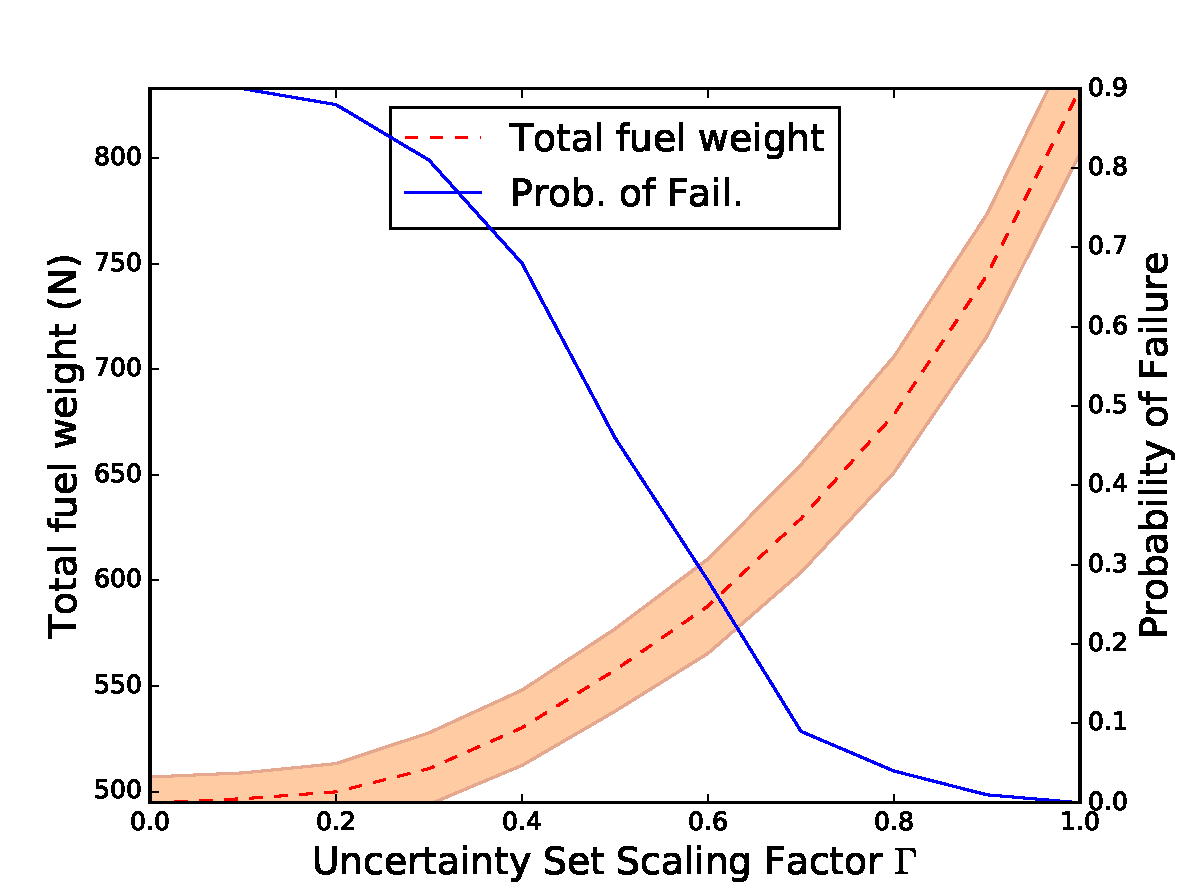
\includegraphics[height=2.3in]{signomial_simple_flight/box_best_pairs.pdf}
         \caption{Box Uncertainty Set}
    \end{subfigure}%
    ~ 
    \begin{subfigure}{0.49\textwidth}
        \centering
        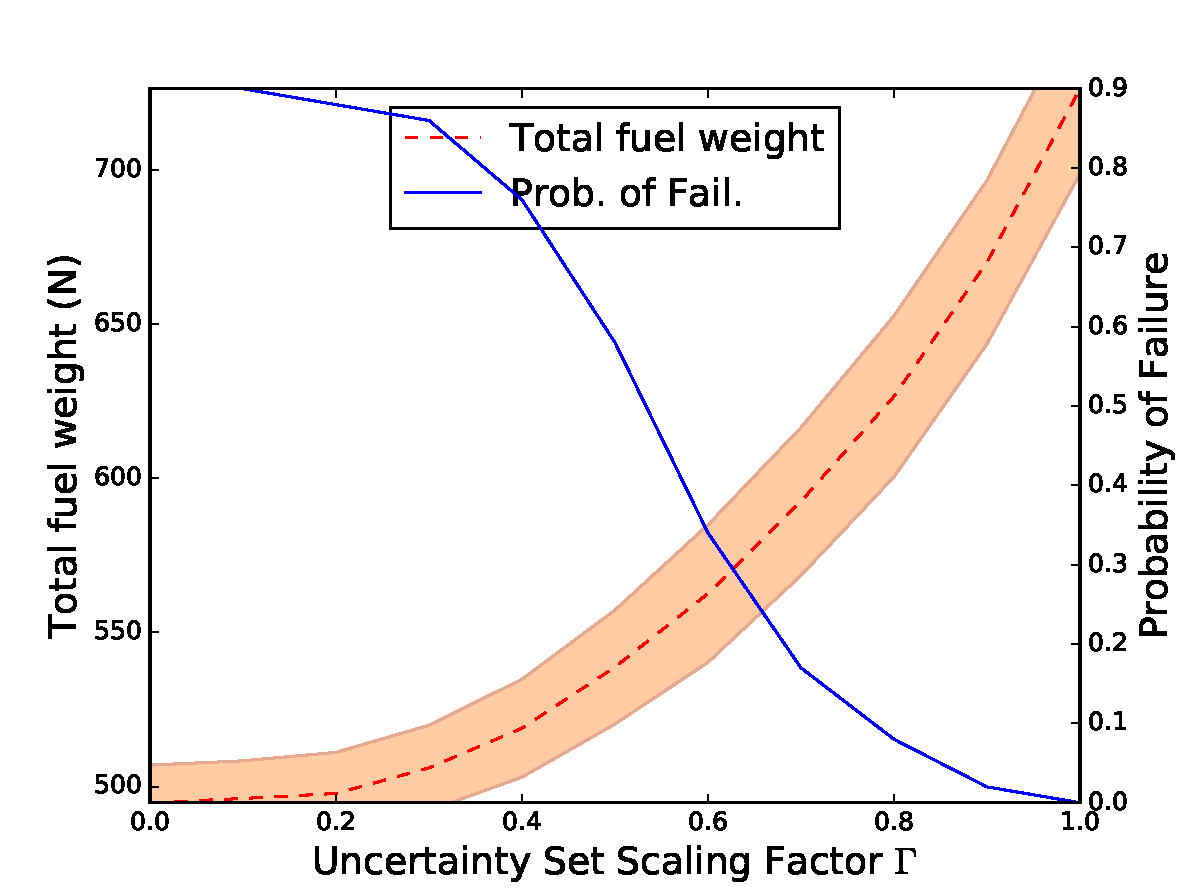
\includegraphics[height=2.3in]{signomial_simple_flight/ell_best_pairs.pdf}
         \caption{Elliptical Uncertainty Set}
    \end{subfigure}
    \caption{Simulated performance of the optimal robust aircraft, using the Best Pairs formulation,
    as a function of $\Gamma$ for different uncertainty sets.
    The dashed line and the band represent the mean and standard deviation of the performance
    of aircraft designed for different $\Gamma$,
    and simulated with 100 \gls{mc} samples of uncertain parameters.}
    \label{fig:probOfFailure}
\end{figure}

We call the aircraft designed under box uncertainty and under elliptical uncertainty `the box aircraft'
and `the elliptical aircraft' respectively. We
define the probability of failure of a design as the probability that any constraint
in the design optimization problem is violated in a \gls{mc} simulation.
As expected, Figure \ref{fig:probOfFailure} shows that probability of failure goes monotonically
to zero as $\Gamma$ increases. However, it is not smooth in its second derivative due to the
presence of the non-log-convex fuel constraint.
It is noteworthy that, for the nominal problem ($\Gamma = 0$) only about 10 percent of the realizations of
uncertain variables result in feasible solutions.
This means that an aircraft designed for the average case would almost surely
fail to satisfy the mission requirements, even with equal likelihood of favorable versus
unfavorable uncertain outcomes from the symmetric truncated Gaussian.
That being said, depending on the problem, it may necessary to sacrifice
performance to achieve a high degree ($3\sigma$) of
reliability as in the solution for $\Gamma = 1$. As shown by Figure~\ref{tab:results},
the elliptical aircraft spends 74\% more fuel
in the worst case than the aircraft designed for the nominal case, but it
is also completely robust to all uncertain outcomes in the $3\sigma$ set.

\begin{table}[!h]
\begin{center}
\caption{\label{tab:results} SP Aircraft Optimization Results}
\begin{tabular}{c c c c c c}
\hline
Free variable & Description & Units & No Uncert. & Box [$\Gamma = 1.0$] & Elliptical [$\Gamma = 1.0$] \\
\hline
$L/D$ & mean lift-to-drag ratio & - & 33.6 & 25.1 & 27.7 \\
$AR$ & aspect ratio & - & 24.6 & 13.0 & 16.3 \\
$Re$ & Reynolds number & - & $1.54 \times 10^6$ & $3.03\times 10^6$ & $250 \times 10^6$ \\
$S$ & wing planform area &$\mathrm{m^2}$ & 13.6 & 32.0 & 28.1 \\
$V$ & mean flight velocity &$\mathrm{m/s}$ & 41.6 & 38.9 & 38.4 \\
$T_{\rm{flight}}$ & time of flight & $\mathrm{hr}$ & 20.1 & 21.4 & 21.7 \\
$W_{\rm{w}}$ & wing weight & $\mathrm{N}$ & 2830 & 4800 & 4480 \\
$W_{\rm{w,strc}}$ & wing structural weight &$\mathrm{N}$ & 2010 & 2670 & 2620 \\
$W_{\rm{w,surf}}$ & wing skin weight &$\mathrm{N}$ & 820 & 2120 & 1860 \\
$W_{\rm{fuse}}$ & fuselage weight &$\mathrm{N}$ & 250 & 288 & 279 \\
$V_{\rm{f,avail}}$ & total fuel volume & $\mathrm{m^3}$ & 0.0759 & 0.154 & 0.136 \\
$V_{\rm{f,fuse}}$ & fuselage fuel volume & $\mathrm{m^3}$ & 0.0394 & 0 & 0.0159 \\
$V_{\rm{f,wing}}$ & wing fuel volume &$\mathrm{m^3}$ & 0.0365 & 0.154 & 0.120    \\
\hline
E[Objective] & Description & Units & No Uncert. & Box [$\Gamma = 1.0$] & Elliptical [$\Gamma = 1.0$] \\
\hline
$W_{\rm{fuel}}$ & total fuel weight & $\mathrm{N}$ & 608 & 1240 & 1090 \\
\hline
P[failure] & & & No Uncert. & Box [$\Gamma = 1.0$] & Elliptical [$\Gamma = 1.0$] \\
\hline
\% & & & 92 & 0 & 0\\
\hline
\end{tabular}
\end{center}
\end{table}

Moreover, using margins in design is similar to using a box uncertainty set, and therefore will lead
to a more conservative solution with inferior performance. This can be seen by the fact that
the elliptical aircraft spends 14\% lower fuel in the worst case
than the box aircraft, although they both protect against the same uncertain outcomes.
The significance of this cannot be understated: the use of margins or box uncertainty protects
against the same amount of risk as elliptical uncertainty, with strictly worse performance outcomes.

In absolute
terms, the nominal \gls{sp} under zero uncertainty
takes just under 0.9 seconds to solve on a modern laptop computer; the authors
refer to ~\cite{Kirschen2018Log} and \cite{York2018} for more in-depth \gls{sp} solution time analyses.
Here we examine briefly in relative terms about how the different \gls{rsp} methodologies compare in terms of setup and
run times in Figure~\ref{compare_signomial}. Since the setup time of the nominal problem is minimal,
we have normalized the results by the run time of the nominal problem.
The bottom axis ranks the methods by their level of conservativeness, Best Pairs
and Simple Conservative formulations being the least and most conservative respectively,
and where the elliptical formulations are less conservative than the box formulations.
For the box uncertainty, solution times are almost identical for different levels of conservativeness,
whereas for the elliptical uncertainty they decrease as the method becomes more conservative.

\ \\
\begin{figure}[ht]
    \centering
    \captionsetup{justification=centering, font=small}
    \begin{subfigure}{0.49\textwidth}
        \centering
        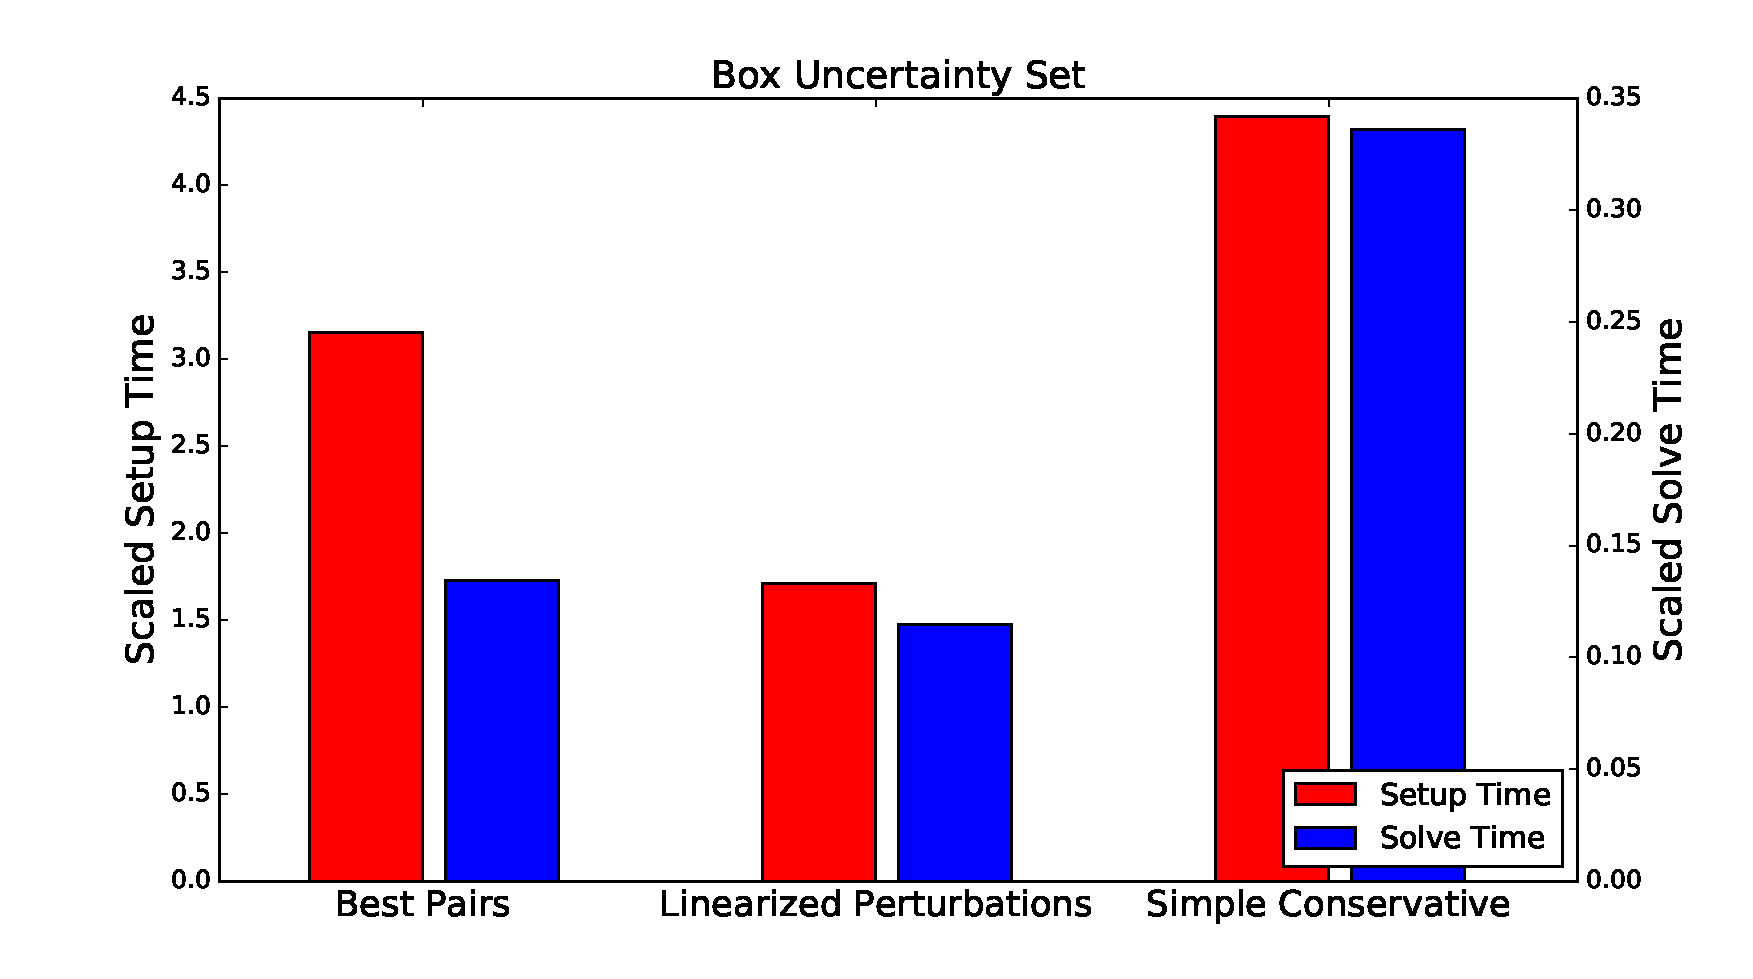
\includegraphics[height=2.3in]{signomial_simple_flight/box_sst.pdf}
    \end{subfigure}
    ~
    \begin{subfigure}{0.49\textwidth}
        \centering
        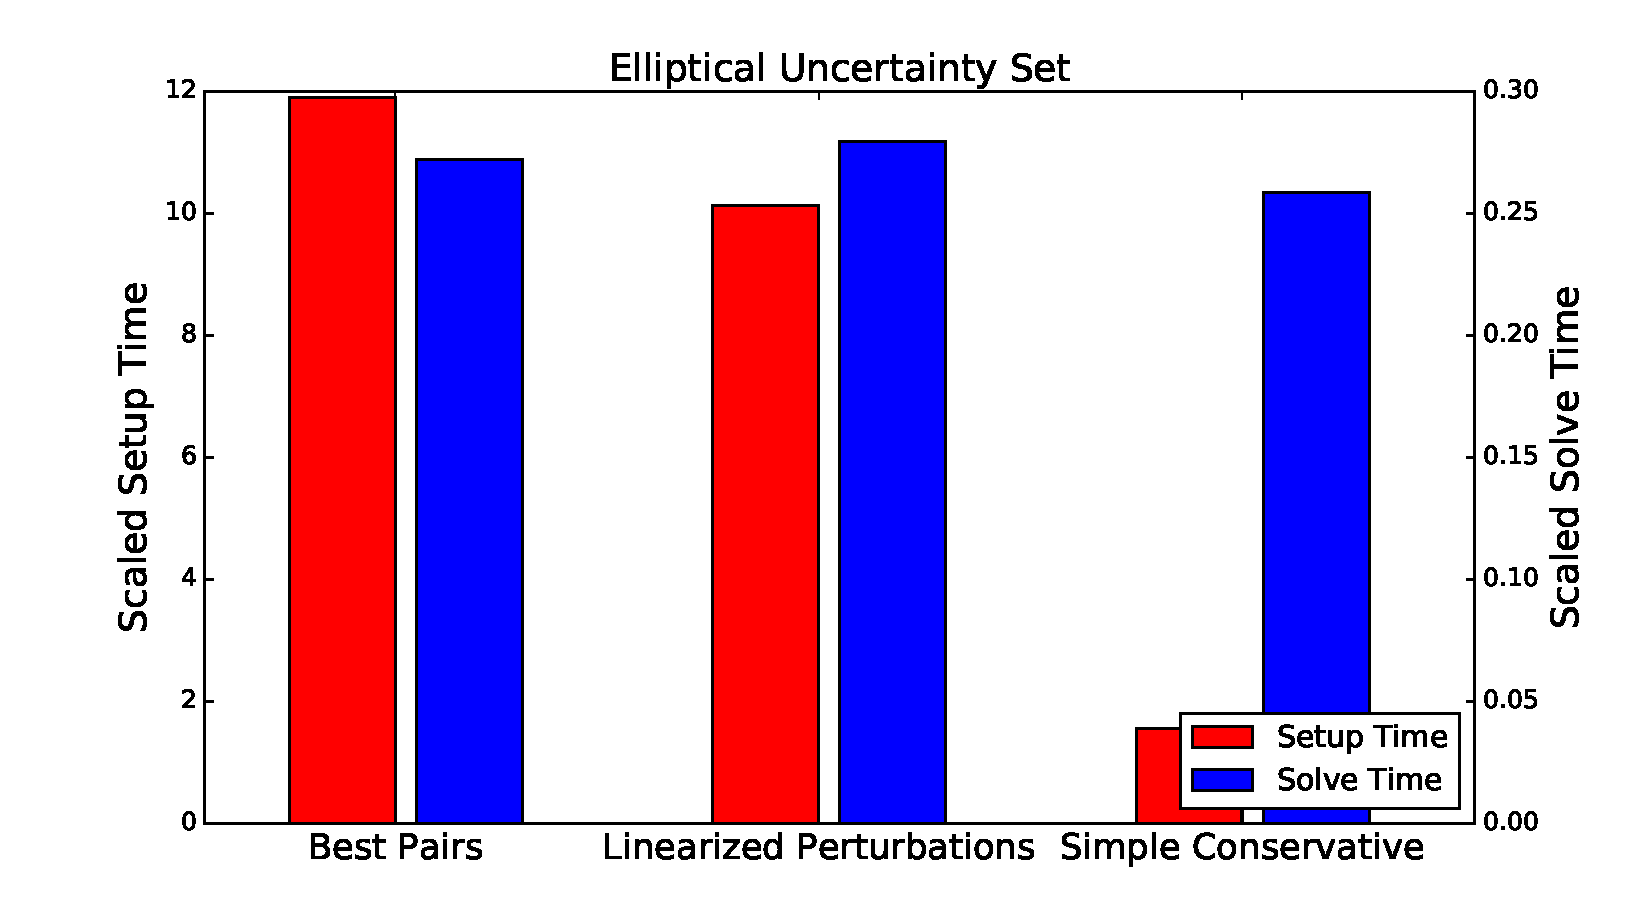
\includegraphics[height=2.3in]{signomial_simple_flight/ell_sst.pdf}
    \end{subfigure}
    \caption{Robust signomial simple aircraft solution and setup times, normalized by the
    nominal problem solution time, for $\Gamma = 1$.
    Note that the problems with box uncertainty have much lower setup
    time costs versus those with elliptical uncertainty, but similar solve times.}
    \label{compare_signomial}
\end{figure}

\subsection{The Effect of Robustness on Multiobjective Performance}

One of the benefits of convex and difference-of-convex optimization methods is the ability to optimize for
different objectives~\cite{York2018}. As a demonstration, we optimize the aircraft without uncertainty
for 8 different objectives, and show
the non-dimensionalized results in Table~\ref{tab:nondimresults}.
Since the model is physics based, the model can even accommodate objectives such as aspect ratio
which are unintuitive and often not considered. The resulting aircraft
differ drastically with respect to performance and design variables.
As the most extreme example,
the aircraft optimized for time cost has more than 100 times the engine weight as the aircraft
optimized for total fuel, since a huge amount of power is required to fly fast. Furthermore, we can see
that some more traditional objectives such as wing loading pull the design
towards extreme corners of the performance envelope. This shows the importance of considering many objectives
in design, and demonstrates the power of \gls{sp}s in helping
consider the multiobjective performance engineered systems.

\begin{table}
    \resizebox{\textwidth}{!}{
    \csvautobooktabularcenter{figures/objective_table.csv}
    }
\caption{Non-dimensionalized variations in objective values with respect to the aircraft optimized
for different objectives. Objective values are normalized by the total fuel solution.}
    \label{tab:nondimresults}
\end{table}

Aside from this caricature example, we demonstrate the capabilities of \gls{rsp}s
by considering a more realistic scenario, now with uncertainty.
We perform the optimization of the aircraft with no uncertainty and both box and
ellipsoidal uncertainty ($\Gamma = 1$)
for 4 different objective functions, and plot the results on spider plots.
Spider plots are useful because they allow engineers to see the performance of
different designs in a multi-objective
environment. One way to envision the multi-objective
performance of the aircraft is to consider the area contained within the web defined by the aircraft's
performance as the figure of merit; the smaller the web area the better.
Due to the large disparities in the potential values of design variables depending
on objective as shown in Table~\ref{tab:nondimresults}, we choose to demonstrate this using four objective functions
that would be expected to have a high degree of correlation and therefore could yield a
nuanced comparative analysis. These are
total (time and fuel) cost, total fuel, takeoff weight and mid-cruise lift-over-drag (L/D).

\begin{figure}
    \begin{center}
    \begin{tikzpicture}
        \node[inner sep=0] (center) at (0,0)
        {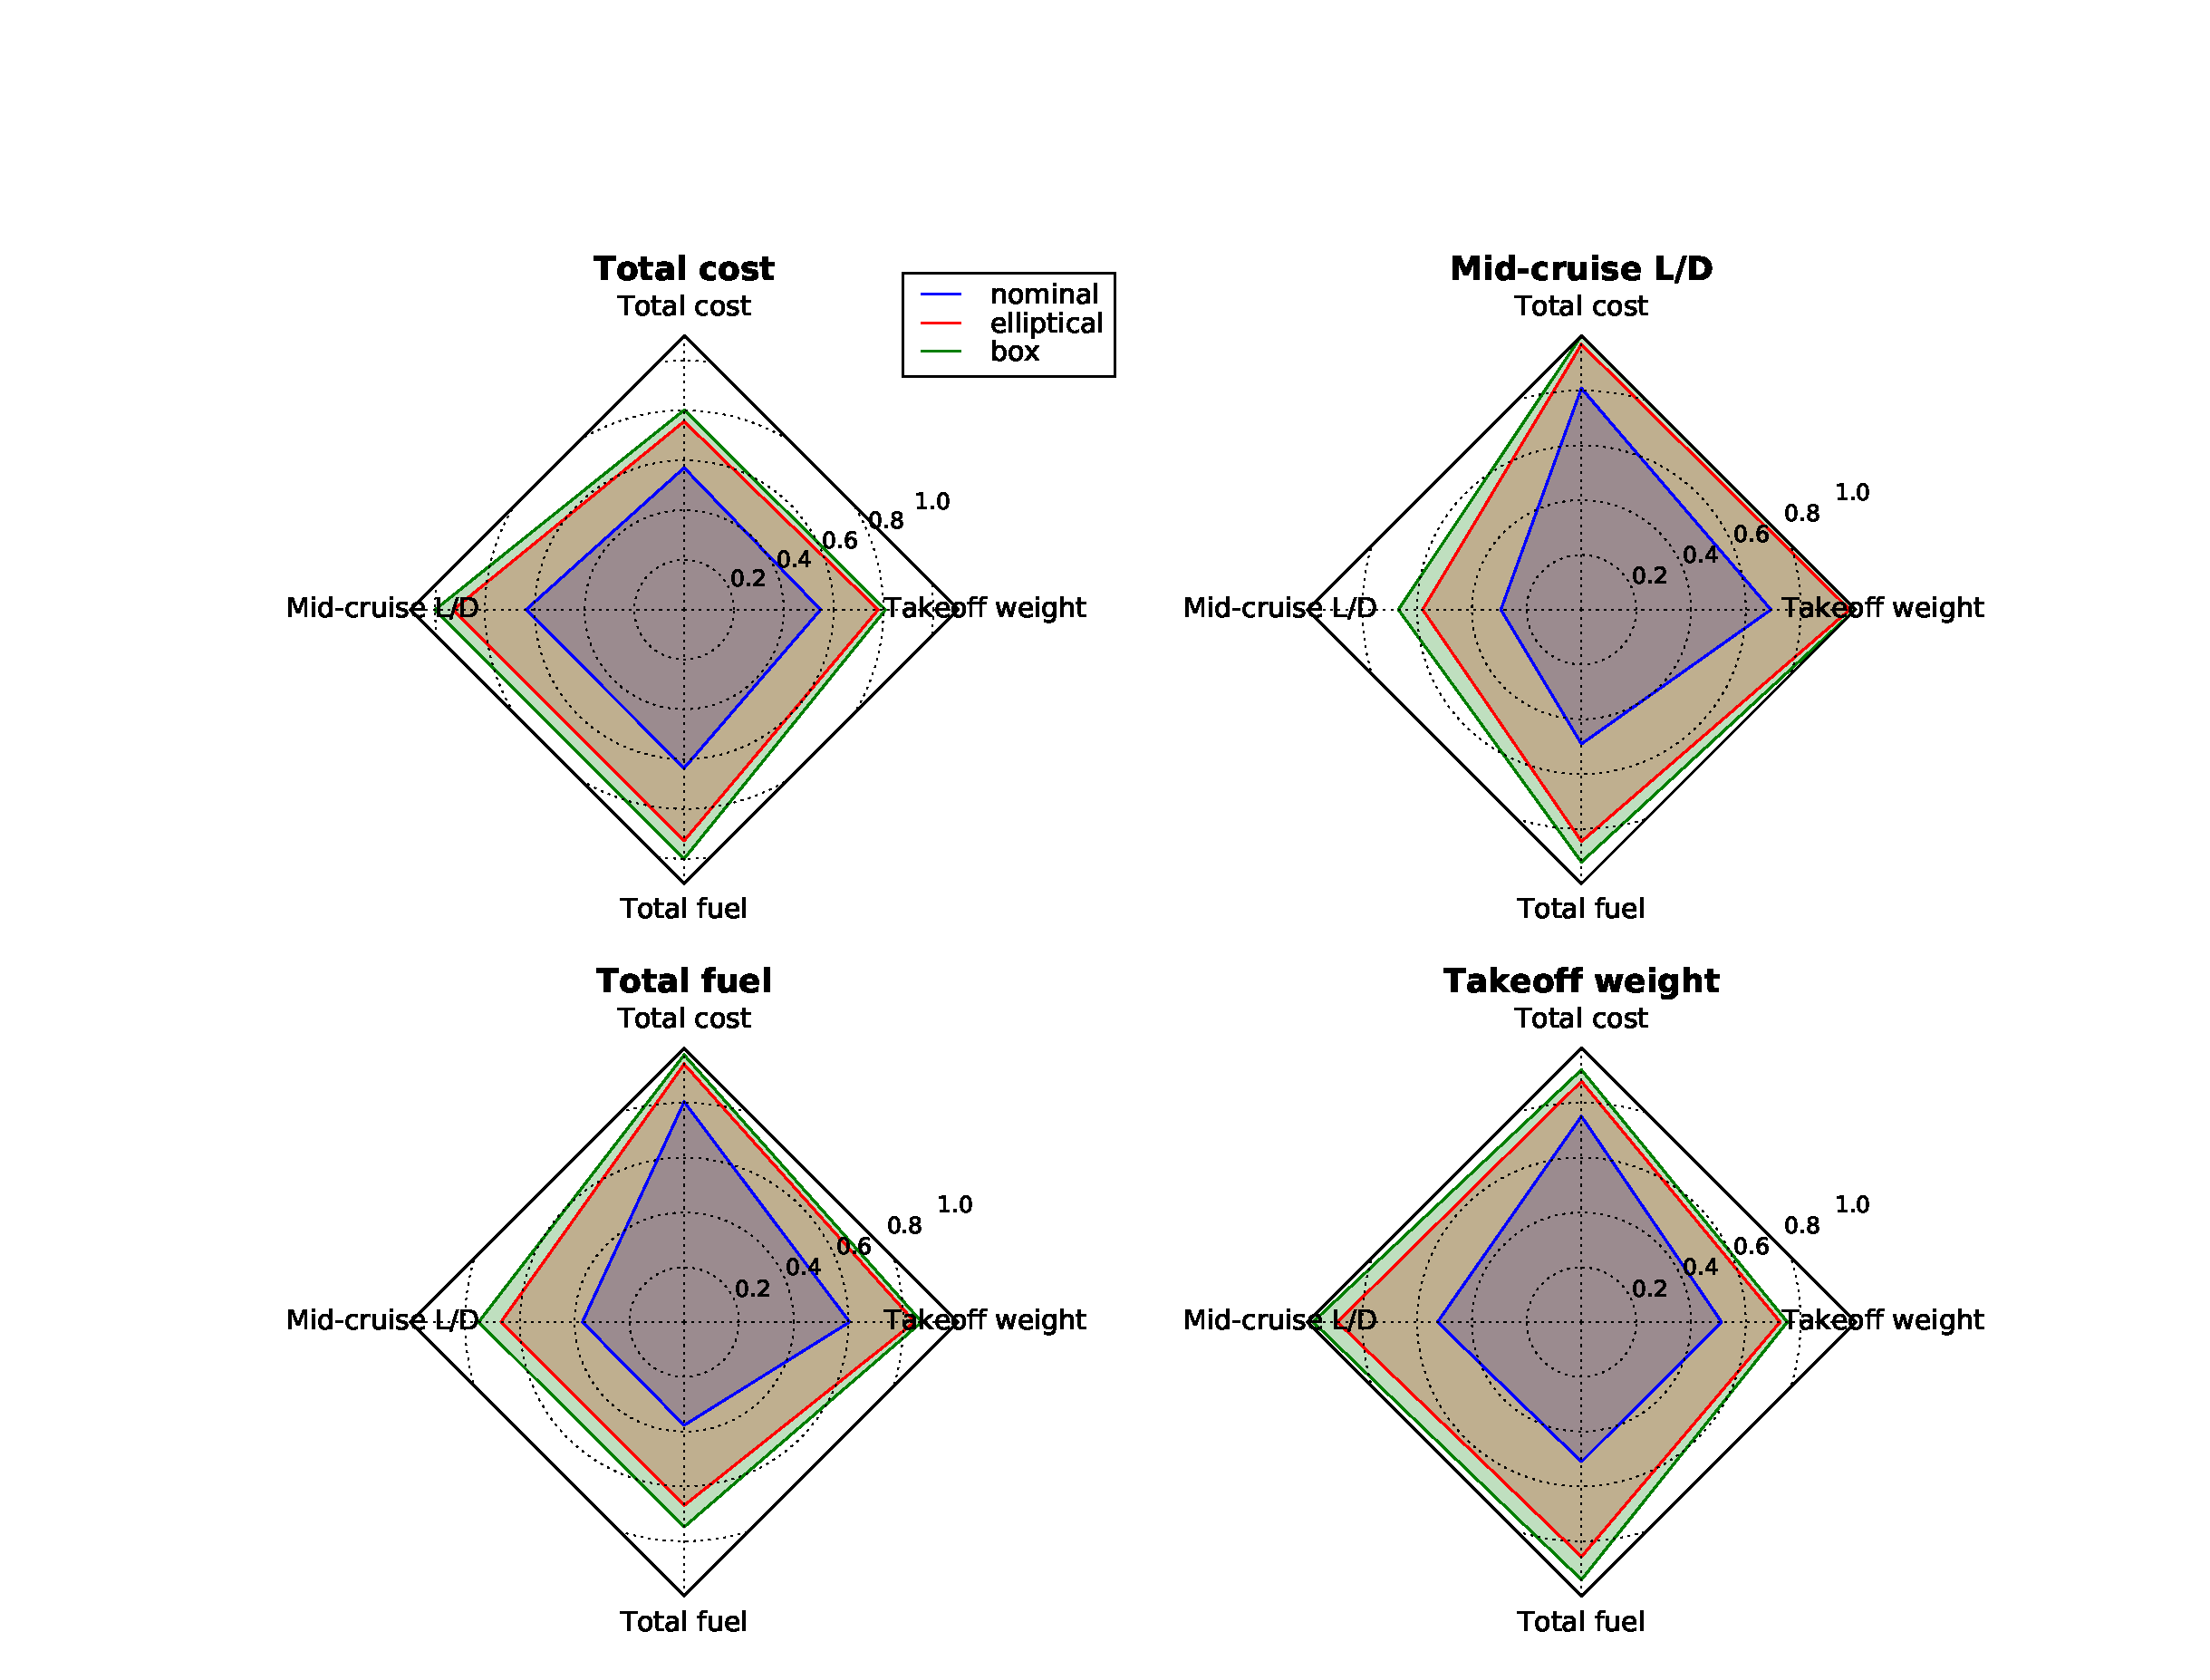
\includegraphics[trim={2cm 0 1cm 0},clip]{figures/4objradar.pdf}};
        \node[inner sep=0] (ul) at (-1.0, 0.25)
        {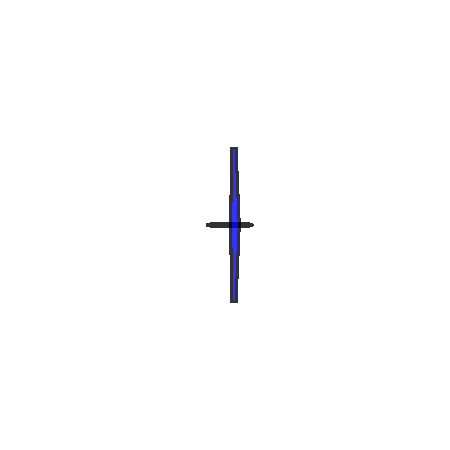
\includegraphics[height=3.8cm]{figures/0nominal.pdf}};
        \node[inner sep=0] (ur) at (1.0, 0.25)
        {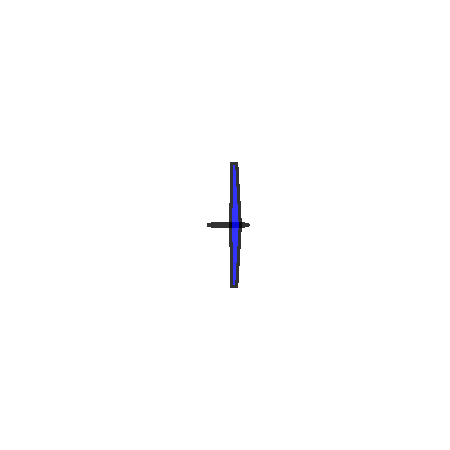
\includegraphics[height=3.8cm]{figures/1nominal.pdf}};
        \node[inner sep=0] (ll) at (-1.0, -2)
        {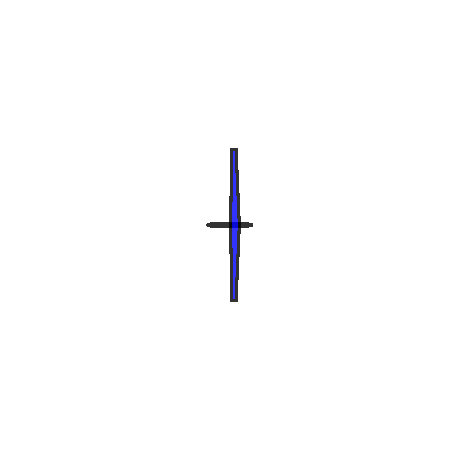
\includegraphics[height=3.8cm]{figures/2nominal.pdf}};
        \node[inner sep=0] (lr) at (1.0, -2)
        {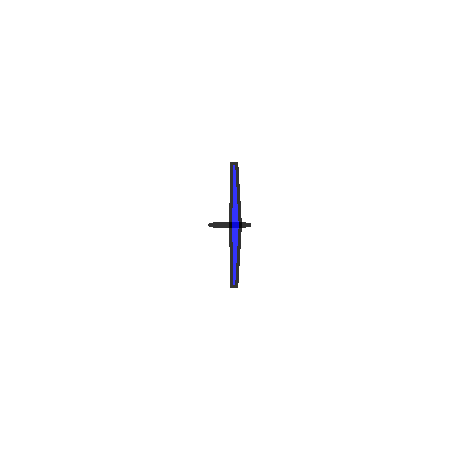
\includegraphics[height=3.8cm]{figures/3nominal.pdf}};
    \end{tikzpicture}
    \caption{The spider plots of aircraft performance, for aircraft optimized for different objectives.
    The bolded titles are the design objectives for each plot, whereas the individual spiderwebs
    show the non-dimensionalized multiobjective performance of the aircraft designed under different
    uncertainty sets. Nominal aircraft shown for comparison. }
    \label{fig:spider}
\end{center}
\end{figure}

\begin{figure}
    \begin{center}
        \begin{subfigure}{0.4\linewidth}
            \makebox[\textwidth]{\begin{tikzpicture}
                \node[inner sep=0] (l) at (-2.5,0)
                {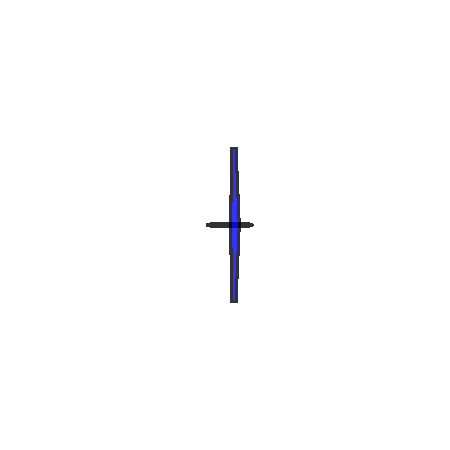
\includegraphics[height=5cm]{figures/0nominal.pdf}};
                \node[inner sep=0] (c) at (-1,0)
                {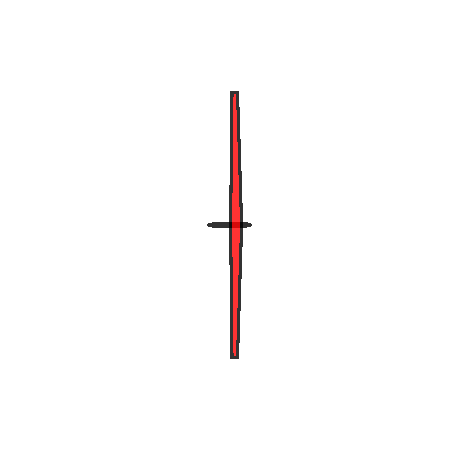
\includegraphics[height=5cm]{figures/0elliptical.pdf}};
                \node[inner sep=0] (r) at (.5,0)
                {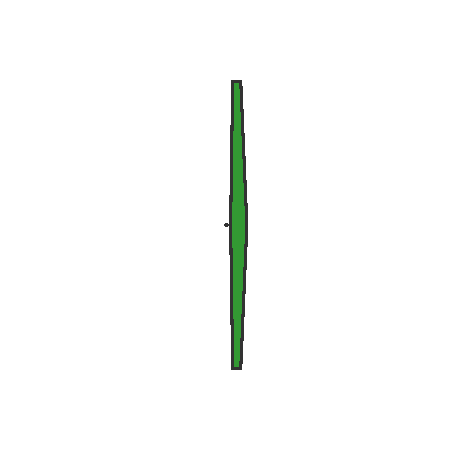
\includegraphics[height=5cm]{figures/0box.pdf}};
            \end{tikzpicture}}
            \caption{Total fuel}
        \end{subfigure}
        \begin{subfigure}{0.4\linewidth}
            \makebox[\textwidth]{\begin{tikzpicture}
                \node[inner sep=0] (l) at (-2.5,0)
                {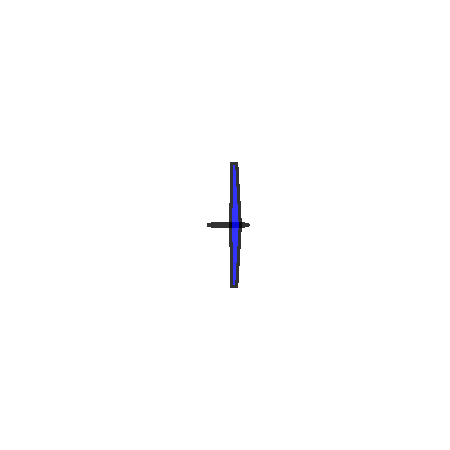
\includegraphics[height=5cm]{figures/1nominal.pdf}};
                \node[inner sep=0] (c) at (-1,0)
                {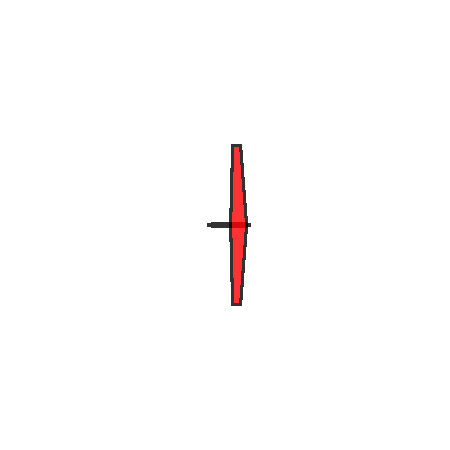
\includegraphics[height=5cm]{figures/1elliptical.pdf}};
                \node[inner sep=0] (r) at (.5,0)
                {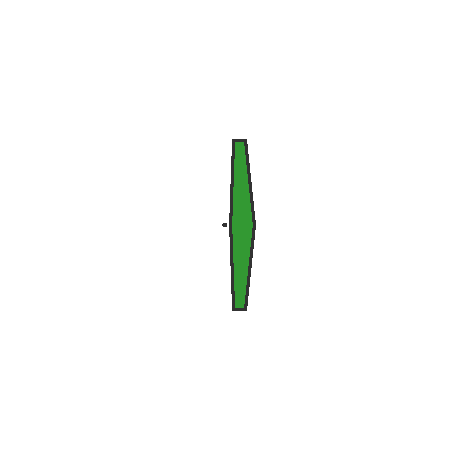
\includegraphics[height=5cm]{figures/1box.pdf}};
            \end{tikzpicture}}
            \caption{Takeoff weight}
        \end{subfigure}
        \begin{subfigure}{0.4\linewidth}
            \makebox[\textwidth]{\begin{tikzpicture}
                \node[inner sep=0] (l) at (-2.5,0)
                {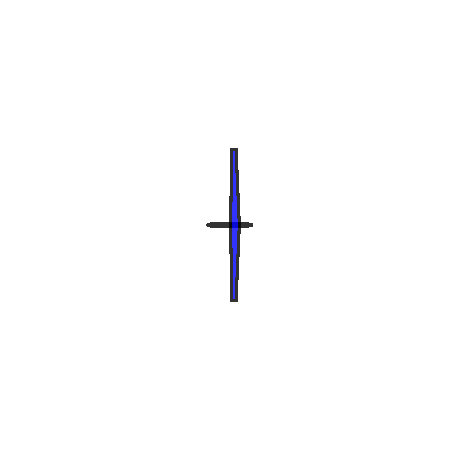
\includegraphics[height=5cm]{figures/2nominal.pdf}};
                \node[inner sep=0] (c) at (-1,0)
                {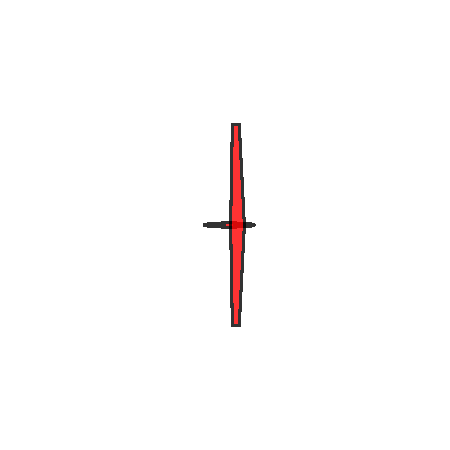
\includegraphics[height=5cm]{figures/2elliptical.pdf}};
                \node[inner sep=0] (r) at (.5,0)
                {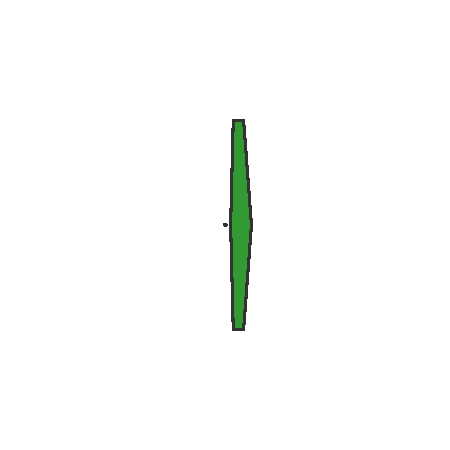
\includegraphics[height=5cm]{figures/2box.pdf}};
            \end{tikzpicture}}
            \caption{Total cost}
        \end{subfigure}
        \begin{subfigure}{0.4\linewidth}
            \makebox[\textwidth]{\begin{tikzpicture}
                \node[inner sep=0] (l) at (-2.5,0)
                {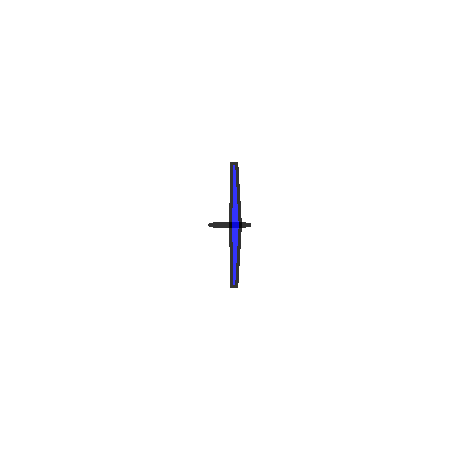
\includegraphics[height=5cm]{figures/3nominal.pdf}};
                \node[inner sep=0] (c) at (-1,0)
                {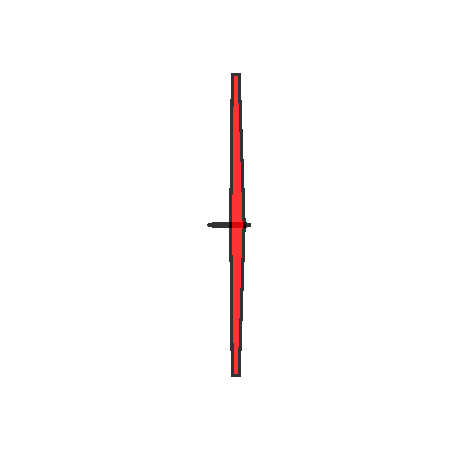
\includegraphics[height=5cm]{figures/3elliptical.pdf}};
                \node[inner sep=0] (r) at (.5,0)
                {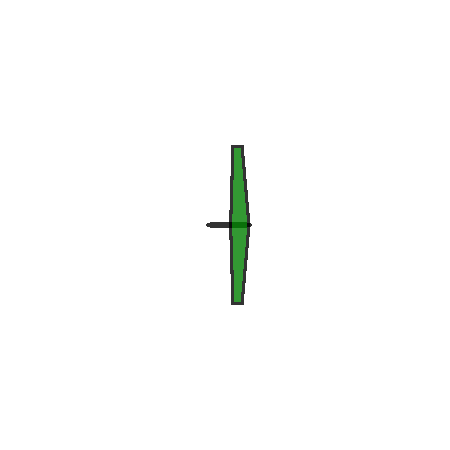
\includegraphics[height=5cm]{figures/3box.pdf}};
            \end{tikzpicture}}
            \caption{Mid-cruise L/D}
        \end{subfigure}
        \caption{Sketches of the aircraft drawn for corresponding spider plots. Drawn to scale for comparison.}
    \end{center}
\end{figure}

Figure~\ref{fig:spider} shows the effects of robustness on
the different worst-case performance metrics of the different aircraft.
For the nominal case, it is possible to see that
the aircraft designed for total fuel performs the best when all four objectives are considered,
assuming that all objectives are weighted equally. As expected,
the box uncertainty set is strictly more conservative than the elliptical uncertainty set for
all objectives. Note that the spider plots show the worst-case performance of the vehicles.
This analysis can also be performed for the mean performance
of the aircraft determined through ~\gls{mc} simulation, but this demonstration limits
its scope to the worst-case analysis.

Based on these observations, we argue that there could be significant value left on the table
if uncertainty is not considered with sufficient mathematical rigor in early phases of
the engineering design process. \gls{rsp}s allow engineers to capture complex
tradeoffs in nonlinear optimization problems while considering uncertainty,
resulting in \emph{less conservative} solutions
than solutions that implement margins and other less rigorous methods for risk mitigation.
Thus \gls{rsp}s improve significantly on the
the paradigms of design under uncertainty in use
in the aerospace industry today.

\subsection{Risk minimization problems}

All of the previous multi-objective analyses have assumed that we have an
understanding of exactly the amount of uncertainty we are
willing to tolerate. However, minimizing risk can also be the objective of our
model. This would suggest the following formulation:

\begin{align}
    \begin{split}
    \text{max} &~\Gamma \\
    \text{s.t.}     &~f_i(x,u) \leq 0, i = 1,\ldots,n \\
                    & \norm{u} \leq \Gamma \\
                    &~f_0(x) \leq (1+\delta)f_0^*,~\delta \geq 0
    \end{split}
    \label{eq:goalprogramming}
\end{align}

where $f_0^*$ is the optimum of the nominal problem in Formulation~\ref{eq:normform} and $\delta$
is a fractional measure of the objective that we are willing to sacrifice for robustness, which
gives $(1+\delta)f_0^*$ as the upper bound on the objective value. Intuitively,
this is a form of goal programming,
where we specify the exact maximum worst-case value of an objective we can tolerate with
the goal of maximizing the total size of the uncertainty $\Gamma$ we can handle.

The goal programming problem in Formulation~\ref{eq:goalprogramming} is clearly
not equivalent to the problem in Formulation~\ref{eq:normform},
but should yield the same results if the method is optimal.
To show this optimality, we will use the objective values from the probability of failure study
shown in Figure~\ref{fig:probOfFailure} as the $\delta$ inputs to the goal programming model, and compare the results.
We expect that $\Gamma$ and $\delta$  from both problems are identical if the method is optimal.
The results are tabulated in
Table~\ref{tab:deltaVsGamma}. Note that the two methods were evaluated \gls{mc} runs using the same 100 realizations
of the uncertainty, for consistency in probability of failure results.

\begin{table}
\begin{center}
\caption{\label{tab:deltaVsGamma} Results of original \gls{ro} problem versus goal program in terms
of size of uncertainty set $\Gamma$, objective penalty $\delta$, and probability of failure. Both methods
use the Best Pairs formulation under elliptical uncertainty. The designs obtained through
the two different methods match.}
\begin{tabular}{c c c c c c c c}
\hline
 \gls{ro} form & $\Gamma$ & $\delta$ & PoF & Goal form & $\delta$ & $\Gamma$ & PoF\\
\hline
& 0.00 & $2.5 \times 10^{-4}$ & 0.94 & & - & - & - \\
& 0.10 & 0.057 & 0.87 & & 0.057 & 0.10 & 0.87 \\
& 0.20 & 0.118 & 0.76 & & 0.118 & 0.20 & 0.76 \\
& 0.30 & 0.183 & 0.60 & & 0.183 & 0.30 & 0.60 \\
& 0.40 & 0.252 & 0.38 & & 0.252 & 0.40 & 0.38 \\
& 0.50 & 0.326 & 0.20 & & 0.326 & 0.50 & 0.21 \\
& 0.60 & 0.406 & 0.10 & & 0.406 & 0.60 & 0.10 \\
& 0.70 & 0.492 & 0.07 & & 0.492 & 0.70 & 0.07 \\
& 0.80 & 0.583 & 0.04 & & 0.583 & 0.80 & 0.04 \\
& 0.90 & 0.681 & 0.01 & & 0.681 & 0.90 & 0.01 \\
& 1.00 & 0.787 & 0.00 & & 0.787 & 1.00 & 0.00 \\
\end{tabular}
\end{center}
\end{table}

Firstly, note that there are no results reported for the smallest uncertainty set $\Gamma = [0.00]$.
Since the feasible set of this problem is a point design, the signomial program
solution heuristic declares the problem infeasible after being
unable to locate the singular feasible region.
Otherwise, the $\Gamma$ values found by the goal programming method match exactly
with the original \gls{ro} method. We confirm that both methods produce
the same designs by examining the physical dimensions of the aircraft, and through the probability
of failure found through \gls{mc} simulation in Table~\ref{tab:deltaVsGamma}.
Note that there is a small discrepancy
in the probability of failure, notably in the value for $\Gamma = 0.5$. This is
because there are uncertainty realizations that can fall
in or out of feasibility due to numerical precision
since the interior point solvers used cannot make computations exactly~\cite{Nesterov1994}.

We can also expand this framework to perform multivariate goal programming,
by changing Formulation~\ref{eq:goalprogramming} to include all
objectives we are interested in.

\begin{align*}
    f_{0,j}(x) \leq (1+\delta_j) f^*_{0,j},~\delta_j \geq 0,~j = 1,\ldots, m
    \label{eq:multigoal}
\end{align*}

The benefit of goal programming is that it allows us to explore multidisciplinary tradeoffs without
having to enumerate the design space along each objective direction.
In design it is not obvious whether an objective should in fact be a constraint instead. The most
fundamental choice that an engineer can make in design is what the objective function is, and it is
often the case that there are many potential objectives that are conflicting.
The term multiobjective optimization is misleading
because you can only optimize for one objective at once,
and the design is going to be influenced by how engineers weigh different objectives.
But risk is ubiquitous in engineering design problems, so goal programming allows risk to be used as
a global design variable against which all objectives can weighed.

\section{Potential Future Work or Studies}

There are a myriad of potential extensions to signomial programming under uncertainty.
In the spirit of helping reduce program risk in aerospace design,
the authors make a few observations and recommendations.

In this study, we do not discriminate between the kinds of constraints violated. However, it would
be possible to rank the severity of constraint violations so as to penalize some (eg. structural safety)
more heavily than others (maximum range constraint). This would inject further realism into the
design under uncertainty since some violations contribute to program risk more
strongly than others.

Another potentially valuable extension to the proposed framework is the concurrent implementation
of multiple sets to contain the uncertain parameters, with the purpose of restricting uncertain
outcomes further. One example of this would be to impose an  L1-norm on the integer number of uncertain parameters
as well as an L2-norm on the overall size of uncertainty set
This method can be used to set the total size of the uncertainty set in a Euclidian sense,
but then also to restrict the stochasticity to a subset of all of the uncertain parameters,
thereby somewhat restricting nature. This also turns the problem into an integer robust
optimization problem which poses interesting computational challenges.

With respect to interesting studies, \gls{ro} opens up the possibility to discover and analyze the benefits
of adaptable architectures in aircraft design versus more traditional point designs
with mathematical rigor. Some examples of these are modular designs, morphing designs,
adaptively manufactured designs and aircraft families. It is likely that these types of engineered
robustness become more effective at reducing program risk
in presence of uncertainty, since they are more likely
to deliver value under adverse stochastic outcomes.

In situations where there is data available to aid design, \gls{ro} can help explore
the design space while taking into account the stochasticity and noise in the data.
This opens up an array of potential trade studies where engineers can learn about
the exposure of designs to the sparsity and spread of data and attempt to gather
data which best reduces the uncertainty in the performance of optimal designs.
